% !TEX root = ../main.tex
%
\chapter{System Design and Implementation}
\label{sec:system}

A very important part of this thesis is the development of the \ac{SDF}, a lightweight, specialized python framework which supports the automatic creation, annotation and analysis of dialogues through LLMs. In this section we explain in detail the initial requirements for this framework and why already-available alternatives do not fit these requirements (Section \ref{sec:system:requirements}), the system's design and concept (Section \ref{sec:system:design-system}), the prompt templates and strategies used (Section \ref{sec:system:design-prompt}) and finally the actual implementation of the \ac{SDF} (Section \ref{sec:system:implementation}).

\section{Requirements}
\label{sec:system:requirements}

The requirements for the \ac{SDF} were not obtained by standard requirement solicitation procedures.  Thus, no formal document detailing them exists. Instead, they were iteratively solicited during weekly meetings with the wider research team, who ultimately decided on a combination of the below requirements. We denote the \ac{SDF} as "the system" for this section.

Functional requirements:
\begin{enumerate}
	\item The system must support multiple LLM types, with potentially different libraries handling them.
	\item The system must support a conversation with at least two LLM users.
	\item The system must support \acp{SDB} to be given to LLM users.
	\item The system must support the existence and absence of a third LLM user, posing as a moderator.
	\item The moderator must be able to intervene at any point in the conversation.
	\item The moderator must be able to "ban" users, preventing them from further commenting.
	\item The output of the system must be serializable and easily parsable.
	\item The system must support automated annotation.
\end{enumerate}

Non-functional requirements:
\begin{enumerate}
	\item The system must be able to be run locally, with scarce computational resources.
	\item The system must be accessed through a simple and flexible \ac{API}.
	\item The system must be able to automatically produce a large amount of synthetic discussions in a timeframe of hours.
	\item The system must support large-scale data annotation.
	\item The system must support a diverse and flexible array of annotation criteria.
\end{enumerate}

Current LLM discussion frameworks such as Concordia \cite{Vezhnevets2023GenerativeAM} and LangChain \cite{langchain} fit, or can be made to fit, all functional requirements listed above. They however fail in almost all non-functional requirements. A major issue is that their \acp{API} are convoluted, although this could be circumvented with enough effort by employing the Adapter pattern \cite{gamma1995design}. Another more serious problem, however, is that their internal components frequently necessitate computer resources (dedicated RAM, GPU VRAM e.t.c.) which, for a smaller application such as ours, will most likely not be used to their fullest. Given that this thesis was developed under acute resource constraints, the latter issue could not be easily resolved.

Thus, the solution of building our own framework is the only practical way of satisfying all the requirements above.



\section{System Design}
\label{sec:system:design-system}

The \ac{SDF} consists of two main functions; \textbf{Synthetic Dialogue Creation} and \textbf{Automatic Dialogue Annotation}. In this section, we will explain how these two functions work conceptually and what their goals are.


\subsection{Synthetic Dialogue Creation}
\label{ssec:system:creation}

We use a simplified version of the LLM discussion framework outlined in \citet{abdelnabi2024cooperationcompetitionmaliciousnessllmstakeholders}. Each actor is given his turn to speak according to a round-robin scheduling algorithm (essentially, each actor takes his turn and passes it to the next actor in line). Each time an actor is prompted to speak, we provide him with a "context window" of \code{h} previous comments in order for him to understand the context of the conversation, where \code{h} is a hyperparameter selected by the experimenter and constrained by the LLM's input context width. Figure \ref{fig::conversation} shows a simplified version of a conversation involving only two users and the moderator. A more general overview of the discussion creation loop can be found in Algorithm \ref{al::dialogue-creation}.


\begin{figure}
	\centering
	\includesvg[width=12cm]{resources/conversation_graph_part4.svg}
	\caption{The conversation loop on which the \ac{SDF} operates. Can be generalized for N users and 0 or 1 moderators.}
	\label{fig::conversation}
\end{figure}

The users and the moderator are all controlled by the same LLM instance (like in \citet{park2022socialsimulacracreatingpopulated}); we only change the system prompt when each takes their turn to speak. The prompts are comprised of five parts:

\begin{itemize}
	\item \textbf{Name}, the name of the actor, used for other actors to refer to him in-conversation.
	\item \textbf{Role}, the role of the actor within the conversation (user or moderator).
	\item \textbf{Attributes}, a list of actor attributes, primarily used for giving the actor an \ac{SDB}.
	\item \textbf{Context}, information known to all users.
	\item \textbf{Instructions}, potentially unique to each actor. 
\end{itemize}


\begin{algorithm}
	\caption{Synthetic Dialogue Creation algorithm} 
	\label{al::dialogue-creation}
	\hspace*{\algorithmicindent} \textbf{Input} users, maxTurns, historyLength\\
	\hspace*{\algorithmicindent} \textbf{Output} the conversation logs
	\begin{algorithmic}[1]	
		\State turn = 0
		\State logs = list()
		\State history = fifo(maxSize=historyLength)
		\State 
		\While{turn < maxTurns}
		\For{user in users}
		\State response = user.speak(history)
		\State logs.add([user.name(), response])
		\State history.add([user.name(), response])
		\State
		\State response = moderator.speak(history)
		\State logs.add([moderator.name(), response])
		\State history.add([moderator.name(), response])
		\EndFor
		\State turn ++
		\EndWhile
		
		\State \Return logs
		
	\end{algorithmic} 
\end{algorithm}



\subsection{Automated Dialogue Annotation}
\label{ssec:system:annotation}

As per the non-functional requirements of Section \ref{sec:system:requirements}, we need a mechanism which can automatically annotate already-executed conversations. This could be achieved by using specialized classification models such as a model for toxicity classification, another for argument quality, and so on. However, these usually differ not only on their exact architecture, but also on their fundamental type; for instance, in toxicity classification, competitive models can be \ac{ML}-based instead of \ac{DL}-based \cite{anjum2024hate}. Using a diverse set of specialized models, with their own libraries, preprocessing requirements and effectiveness would severely restrict our ability to rapidly change annotation criteria at-scale. 

In order to bypass this restriction, we can use LLMs to also handle the annotation step. LLM inference is practically constant-time with a fixed input length, since adding a new annotation metric would only impose a computational penalty equal to the output's increased number of tokens - which is negligible. 

Using LLMs as annotators imposes both a challenge and an opportunity, since annotations are no longer objective (unlike traditional \ac{ML} and even \ac{DL} models, we can't reliably explain a LLM's decision). Thus, we are faced with two different approaches:

\begin{itemize}
	\item Attempt to find a prompt which produces results closer to what would be expected of a human annotator.
	\item Lean into the subjectiveness of LLM decision-making, using many LLM annotators, each with a different \ac{SDB}, and computing their (inter-annotator) agreement.
\end{itemize}

In this thesis, we use the second option.

We re-use the conversation paradigm of Section \ref{ssec:system:creation} to facilitate annotation. One pseudo-actor is the system, which outputs comments made in a conversation one-by-one. The other is a LLM actor, which responds with the classification rating for each comment (toxicity in these experiments).  We use a context window  (\code{h}) for the annotator; in other words, for each comment, the annotator can see the \code{h} preceding comments of the conversation, in order to ensure he understands the context under which each comment was made. The annotation loop is succinctly demonstrated in Figure \ref{fig::annotation} and in Algorithm \ref{al::dialogue-annotation}.

\begin{figure}
	\centering
	\includesvg[width=12cm]{resources/annotation_graph_2.svg}
	\caption{The annotation loop on which the \ac{SDF} operates. Note the purposeful similarity of the procedure to Figure \ref{fig::conversation}.}
	\label{fig::annotation}
\end{figure}

\begin{algorithm}
	\caption{Synthetic Dialogue Annotation algorithm} 
	\label{al::dialogue-annotation}
	\hspace*{\algorithmicindent} \textbf{Input} annotator, logs, historyLength\\
	\hspace*{\algorithmicindent} \textbf{Output} the annotation logs
	\begin{algorithmic}[1]	
		\State annotations = list()
		\State history = fifo(maxSize=historyLength)
		\State 
		\For{message in logs}
		\State history.add(message)
		\State response = annotator.speak(message, history)
		\State annotations.add([message, response])
		\EndFor
		
		\State \Return annotations
	\end{algorithmic} 
\end{algorithm}


\section{Prompt Design}
\label{sec:system:design-prompt}

\subsection{Defining Policy \& Environment}

In order to create convincing prompts for both facilitators and users, we first had to define the rules of the discussion, which necessitated the definition of a policy for our virtual chat-room. We defined this policy according to how an ideal online/deliberative discussion would look like.

As mentioned in Section \ref{sec:related:sec1}, our goal is neither to promote arguments that convince the most people (like in formal debates), nor to necessarily reach consensus or agreement among the participants. The goal of our platform is for the most opinions to be heard by the most people. We have already identified two key inhibitors to this goal; toxicity and personal attacks.

Our facilitator prompts were largely designed on preventing these two phenomena. We also utilize some general guidelines solicited from the Cornell eRulemaking moderator manual \cite{Cornell_eRulemaking2017}:

\begin{itemize}
	\item The moderator must remain neutral and impartial. 
	
	\item Responses should be briefly reflected upon before being posted.
	
	\item Questions posed by the moderator must be purposeful, as if they have one chance to interact with the user. They can rephrase a user's point if they do not understand it.
	
	\item Language should be short and simple.
\end{itemize}

Finally, we discourage the facilitator from intervening too many times. Should this happen, we can reasonably assume that the facilitator's interventions are not effective. An abstract overview of this process can be found in Figure \ref{fig::policy}.

\begin{figure}
	\centering
	\includesvg[width=12cm]{resources/moderator_policy.svg}
	\caption{The procedure with which we created our experimental moderator instructions.}
	\label{fig::policy}
\end{figure}

Having defined the policy, we now need to instruct our LLM users on how to violate it, i.e. we generally want to encourage toxicity and personal attacks. We model their instructions according to how these phenomena occur naturally in online conversations. Specifically:

\begin{itemize}
	\item Many people are unwilling to change opinions during online discussions.
	
	\item Personal attacks are common \cite{dekock2022disagree}.
	
	\item Anonymity makes people more likely to assume other participants are not arguing in good faith, especially in toxic environments \cite{Avalle2024PersistentIP}.
	
	\item People are not told what to believe when entering a discussion, but form opinions based on (besides many other factors) their \ac{SDB}. 
	
\end{itemize}

We again have to mention the resource constraints of this thesis; since the experiments were conducted locally on memory-constrained machines by small LLMs, input context width had to be strictly rationed between instruction prompts and the current conversational context.


\subsection{"Moderation Game" prompts}
\label{ssec:system:game-prompt}

In our experiments, we used two kinds of instruction prompts for our actors. One is a "standard" instruction prompt summarizing the guidelines above. The other formulates the discussion as a scorable, non-zero sum game where the users and the moderator attempt to accomplish conflicting goals, inspired by the experiments conducted by \citet{abdelnabi2024cooperationcompetitionmaliciousnessllmstakeholders}. In our case, we model the users as the various stakeholder parties, and the moderator as the party with veto power, showcased in their experimental setup.

Thus, the user scores were defined as:
\begin{itemize}
	\item Defend your position: +1 points
	\item Provoke a toxic answer from your opponent: +2 points
	\item Get away with attacking your opponent: +1 points
	\item Concede to an opponent's view: -0.5 points
	\item Get banned from the discussion: -20 points
\end{itemize}

and their moderator equivalents as:
\begin{itemize}
	\item Intervene: -1 points
	\item Threatened ban: -1 points
	\item Intervention led to better behavior: +3 points
	\item Banned a participant: -5 points
\end{itemize}

The assigned actions and weights were somewhat arbitrary. In the future, we hope to use \ac{RL} or some selection strategy in order to tune them in a way that is optimal for facilitation, according to synthetic experiments.

\subsection{Annotator prompts}
\label{ssec:system:annotator-prompt}

The annotator prompt consists of the following parts:

\begin{itemize}
	\item The \ac{SDB} prompt.
	
	\item An instruction prompt, in this case geared towards toxicity classification. This part however can be replaced to make the model output any combination of annotations.
	
	\item A list of examples with varying toxicity (few-shot learning).
	
	\item The output prompt.
\end{itemize}

Due to limitations in context window length, the prompt only contained basic information and only a few examples.

\section{Implementation}
\label{sec:system:implementation}

\subsection{Synthetic Discussion Library}
\label{ssec:system:library}

The \ac{SDF} is at its core based on the \ac{SDL} around which the rest of the framework operates. The library is written in Python, contains 4 distinct modules, and is based on \ac{OOP} principles.

Each of these modules contains classes and supporting code for a specific function. In brief:

\begin{itemize}
	\item \textbf{models.py} holds Adapter classes \cite{gamma1995design} which enable the framework to uniformly access almost any LLM instance regardless of type (as long as a suitable subclass is created).
	
	\item \textbf{actors.py} which holds Wrapper classes \cite{gamma1995design}, containing Model Adapter classes from \textbf{models.py} and providing them with prompt templates.
	
	\item \textbf{conversation.py} uses Actor classes in order to execute and serialize the conversation.
\end{itemize}

The library additionally provides the \textbf{annotator.py} and \textbf{util.py} modules, which are self-explanatory.


\subsection{Framework entry-points}
\label{ssec:system:entrypoints}

The framework provides a variety of \acp{API} to access the \ac{SDL} from the more standardized (which necessitate no programming) to the more flexible (direct access to the library's public \ac{API}). These are:

\begin{itemize}
	\item Automated python scripts which, when given a \ac{JSON} configuration file, begin batch production of automated discussions.
	
	\item Jupyter notebooks with explanatory high-level documentation, which are used for on-boarding users to the framework and quick experimentation.
	
	\item The exported \ac{SDL} itself.
\end{itemize}


\subsection{High-level view of the system}
\label{ssec:system:overview}

A high-level overview of the system can be found in Figure \ref{fig::system}. The configurations (\colorSystemConfig{green shapes}) can be provided by either \ac{JSON} files or programmatically, depending on the entry-point (\colorSystemEntrypoint{blue shapes}) used. The actual processing steps (\colorSystemProcessing{pink shapes}) are executed through the \ac{SDL}. The resulting data (\textbf{white shapes}) are then exported as datasets and used in subsequent analyses.

The procedure described in the figure, enables us to produce a large amount of data, annotate them, analyze them, and produce concrete results (graphs, statistical tests e.t.c.) with little-to-no manual intervention. Subsequently, these results enable us to change the prompts used by the Actors to refine results or test new hypotheses.

Each processing step (\colorSystemProcessing{pink shapes}) additionally creates entries on our generated dataset, be it the conversation logs with rich meta-data (\colorSystemProcessing{"Generate Conversation"}), multi-annotator, multidimensional annotations (\colorSystemProcessing{"Generate Annotation"}) or controversial comments (\colorSystemProcessing{"Data Analysis"}).

\begin{figure}
	\centering
	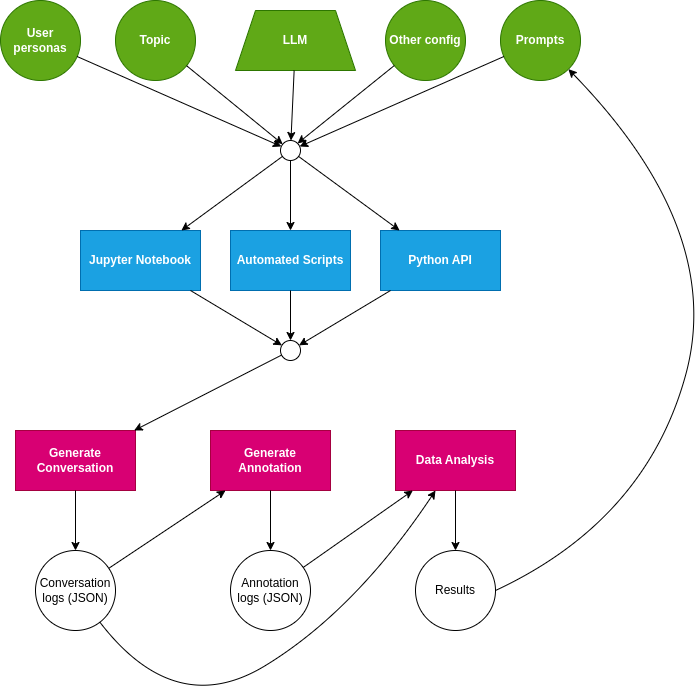
\includegraphics[width=12cm]{system_light.png}
	\caption{An abstract view of the \ac{SDF}. \colorSystemConfig{Green shapes} represent various configurations, \colorSystemEntrypoint{blue shapes} entry points (see Section \ref{ssec:system:entrypoints}), \colorSystemProcessing{pink ones} processes delegated to the \ac{SDL}, and \textbf{white} ones exported data.}
	\label{fig::system}
\end{figure}



\subsection{Technical Details}
\label{ssec:system:details}

The LLM used is the LLaMa2-13B GGUF quantized version. We use the \code{llama\_cpp} python library to load and interact with the model. Details on the environment, software and operating system compatibility, as well as low-level decisions and optimizations, we recommend checking the project's GitHub repository \footnote{\url{https://github.com/dimits-ts/llm_moderation_research}}.

